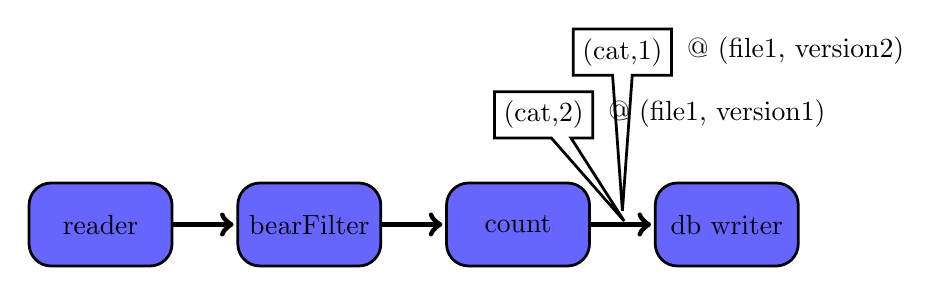
\begin{tikzpicture}[node distance = 0.8cm, auto]
\usetikzlibrary{shapes,arrows}
\usetikzlibrary{positioning}

\tikzstyle{operator} = [rectangle, draw, fill=blue!60, text width=4.5em, text centered, rounded corners = 8pt, minimum height=30pt, line width=1pt]
\tikzstyle{callout} = [draw, rectangle callout, callout relative pointer={#1}, line width=1pt]

    \node [operator] at (0, 0) (reader) {reader};
    \node [operator, right = of reader] (filter) {bearFilter};
    \node [operator, right = of filter] (count) {count};
    \node [operator, right = of count] (writer) {db writer};

    \draw [thick,->,shorten >=1pt, line width=2pt] (reader) -- (filter); 
    \draw [thick,->,shorten >=1pt, line width=2pt] (count) -- (writer) 
       node[callout={(0.8,-30pt)}, midway, shift={(-1,-0.5)}, above = 45pt] {(cat,2)} node[midway,above= 45pt, shift={(1.2,-0.5)}] {@ (file1, version1)}
       node[callout={(0.0,-49pt)}, midway, shift={(0,1)}, above = 25pt] {(cat,1)} node[midway,above= 25pt, shift={(2.2,1)}] {@ (file1, version2)};
     \draw [thick,->,shorten >=1pt, line width=2pt] (filter) -- (count); 
\end{tikzpicture}
